\documentclass{beamer}
% \usepackage{xcolor}
\usepackage{lineno}
\usepackage{minted}
% \usemintedstyle{native}
\usemintedstyle{friendly}
\graphicspath{ {images/} }
\usetheme{boxes}
\setbeamertemplate{blocks}[rounded][shadow=true]

\newenvironment{codeblock}[1]{%
  \setbeamercolor{block body}{bg=white,fg=black}
  \setbeamercolor{block title}{bg=gray,fg=white}
  \begin{block}{#1}}{\end{block}}

\newcommand{\code}[3][]{
  \begin{codeblock}{#2}
  \inputminted[fontsize=\scriptsize,#1]{python}{#3}
  \end{codeblock}
}
\title{My Restful Lab}
\subtitle{Hardware control through a REST API}
\author{Federico Ariza}
\date{\today}

\begin{document}
\begin{frame}
  \titlepage
\end{frame}


\begin{frame}
\frametitle{My hardware}
\begin{figure}
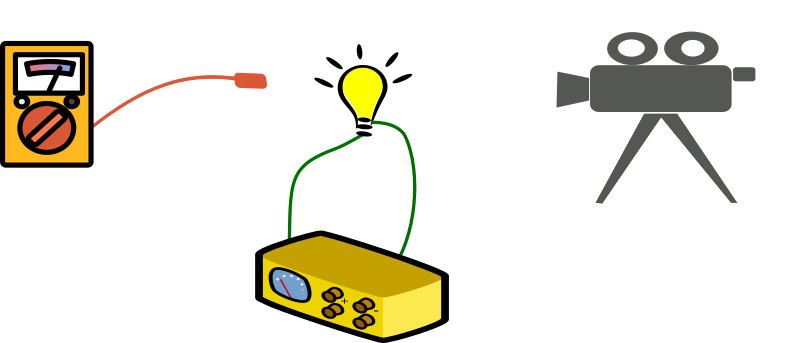
\includegraphics[width=\textwidth]{hw}
% \caption{Power Supply (PSU)}
\end{figure}
\end{frame}

\begin{frame}{Typical test}
  \only<1>{
    \code{Simple test}{code/test.py}
  }
  \only<2>{
    \begin{figure}
    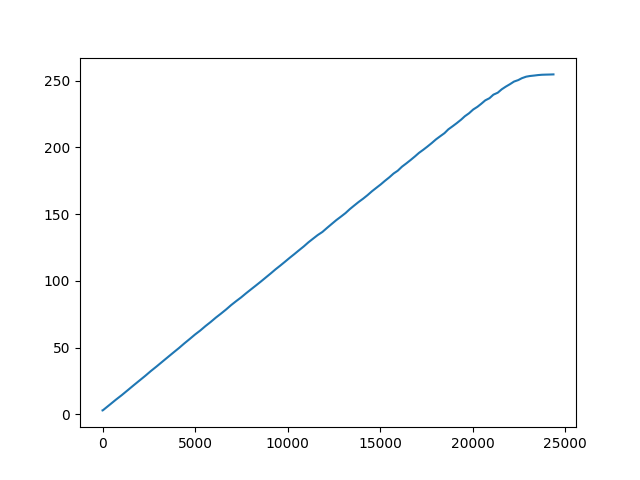
\includegraphics[height=0.8\textheight]{emva_uy}
    \end{figure}
  }
  \only<3>{
    \begin{figure}
    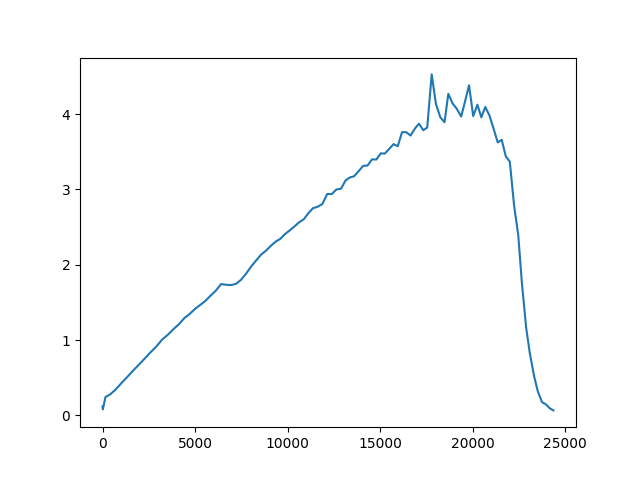
\includegraphics[height=0.8\textheight]{emva_s2y}
    \end{figure}
  }
 
\end{frame}


\begin{frame}{Power Supply (PSU)}
  \code{Basic PSU}{code/psu1.py}
\end{frame}

\begin{frame}{Direct API}
  \begin{block}{Nice}
    \begin{itemize}
      \item Natural interface
      \item It's my interface of choice
      \item It's my language of choice
    \end{itemize}
  \end{block}
  \pause
  \begin{alertblock}{Not so nice}
    \begin{itemize}
      \item User has to be phisically connected to device
      \item That guy over there wants to use C#/lisp?
    \end{itemize}
  \end{alertblock}
\end{frame}

\begin{frame}{Remote API}
  \textbf{Can I "remotisize" my API?}
  \begin{itemize}
    \item Is my API simple enough?
    \item All methods inputs/outputs can be serialized (to strings)?
  \end{itemize}
  \pause
  \vspace{1cm}
  \textbf{What are my options?}
  \begin{itemize}
    \item Handmade socket protocol
    \item RPC
    \item ...
    \item REST
  \end{itemize}
\end{frame}

\begin{frame}
\frametitle{My choice REST}
\begin{figure}
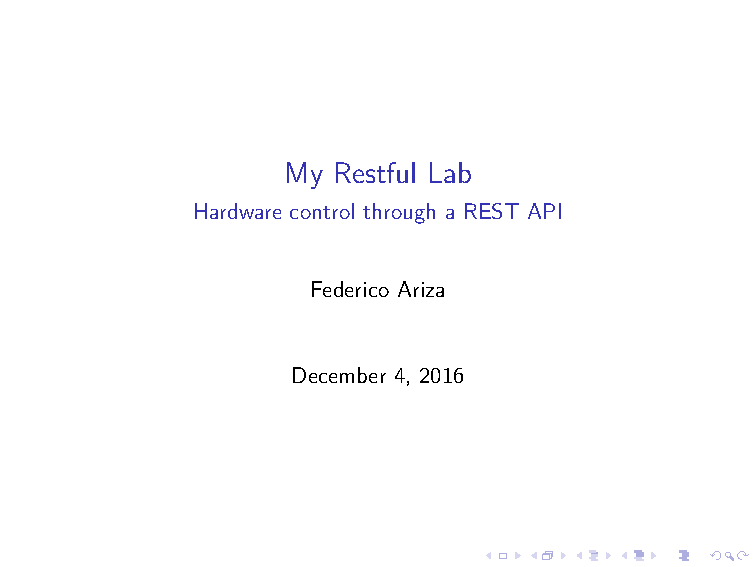
\includegraphics[height=0.8\textheight]{rest}
% \caption{Power Supply (PSU)}
\end{figure}
\end{frame}

\begin{frame}{Rest basics}
  \begin{block}{URL: \textbf{http://hostname:port/zzz/X1/X2/X3}}
    \only<2>{zzz: Base path (webserver config)}
    \only<3>{
      Can have verbs Associated to:
      \begin{itemize}
        \item: X1
        \item: X1/X2
        \item: X1/X2/X3
      \end{itemize}
      }
      \only<4>{
        Can be variables
        \begin{itemize}
          \item X1
          \item X2
          \item X3
        \end{itemize}
      }


      \only<5>{
        \begin{itemize}
          \item Read current: .../current
          \item Read max current: .../psu/current/max
          \item Set current of 5th psu: ../psu/5/current/3.5
        \end{itemize}
      }
      \only<6>{
        Pass Data
        \begin{itemize}
          \item Variable .../current/3.5
          \item Querystring: ?&var1=xx\&var2=yy...
          \item Data inside body: $data=\{var1:x1, var2:x2\}$
        \end{itemize}
      }

  \end{block}

\only<7>{
  \begin{block}{Verbs}
    \begin{itemize}
      \item GET: Read
      \item POST: Create
      \item PUT: Update/Replace
      \item PATCH: Update/Modify
      \item DELETE: Delete
    \end{itemize}
  \end{block}
  }
\only<8>{
\begin{block}{Return Codes}
\begin{itemize}
  \item 200: OK
  \item 201: Created
  \item 404: Not Found
  \item 409: Conflict
\end{itemize}
\end{block}}
\end{frame}

\begin{frame}{My REST API}
\begin{itemize}
  \item GET(http://hostname/voltage) \\ $\rightarrow$ psu.voltage \pause
  \item PUT(http://hostname/voltage, \{'data': value\}) \\ $\rightarrow$ psu.voltage=value
  \pause
  \item PUT(http://hostname/turn\_on, \{\}) \\ $\rightarrow$ psu.turn\_on
\end{itemize}
\end{frame}

\begin{frame}{Rest interface for PSU}
  \only<1>{
    \code[lastline=10]{Flask boilerplate}{code/flask1.py}
  }
  \only<2>{
    \code[firstline=10]{REST}{code/flask1.py}
  }
  % \begin{codeblock}{Rest implementation}
  %   \begin{columns}[T]
  %   \begin{column}{0.5\textwidth}
  %     \inputminted[fontsize=\scriptsize,lastline=19]{python}{code/flask1.py}
  %   \end{column}
  %   \vrule{}
  %   \begin{column}{0.5\textwidth}
  %     \inputminted[fontsize=\scriptsize,firstline=19]{python}{code/flask1.py}
  %   \end{column}
  % \end{columns}
  % \end{codeblock}
\end{frame}


\begin{frame}{Rest client}
  \only<1>{
    \begin{codeblock}{Bash}
      \inputminted[fontsize=\scriptsize]{bash}{code/restclien1.sh}
    \end{codeblock}
  }
  \only<2>{
    \begin{codeblock}{C++}
      \inputminted[fontsize=\scriptsize]{c}{code/restclient1.cpp}
    \end{codeblock}
  }


  \only<3>{
    \code{Python}{code/restclient1.py}
  }

\end{frame}


\begin{frame}
  \begin{block}{Nice}
    \begin{itemize}
      \item Controller and user can be separated
      \item Natural interface
      \item Remote and local interface are the same
      \item User choice of language
    \end{itemize}
  \end{block}
  \pause
  \begin{alertblock}{Not so much}
    \begin{itemize}
      \item THREE (or more)! times the same code
    \end{itemize}
  \end{alertblock}
\end{frame}

\begin{frame}{DRY and SSOT}
\begin{itemize}
  \item Implementation includes extra info (metadata)
  \item Description auto-extracted from Implementation
  \item Server auto-generates from Description
  \item Client auto-generates from Server
\end{itemize}
\end{frame}

\begin{frame}{Add some metadata}
  \code{PSU with extra info}{code/psu2.py}
\end{frame}


\begin{frame}{Use the metadata}
  \code{Get api from code}{code/extractor.py}
\end{frame}

\begin{frame}{Auto server}
  \only<1>{
    \code[lastline=21]{Flask boilerplate}{code/flask2.py}
  }
  \only<2>{
    \code[firstline=21]{Rest resources}{code/flask2.py}
  }
\end{frame}

\begin{frame}{Auto client}
  \only<1>{
    \code[lastline=22]{Init class}{code/restclient2.py}
  }
  \only<2>{
    \code[firstline=24]{Auto attributes and methods}{code/restclient2.py}
  }
\end{frame}

\begin{frame}{What about C/C++ client?}
  \begin{block}{Piece of cake}
    Just call jinja!
  \end{block}
\end{frame}

\begin{frame}[plain]
  \begin{center}
    \Huge Thanks!
  \end{center}
\end{frame}

\end{document}
